\documentclass[11pt]{article}
\usepackage[margin=0.82in]{geometry}
\usepackage[T1]{fontenc}
\usepackage{lmodern}
\usepackage{amsmath,amssymb,amsthm,mathtools}
\usepackage{booktabs,array,enumitem,microtype,graphicx,longtable}
\usepackage{float}
\usepackage{tikz}
\usetikzlibrary{arrows.meta,fit,positioning}
\usepackage[hidelinks]{hyperref}
\usepackage[nameinlink,capitalise]{cleveref}
\usepackage[backend=biber,style=numeric,sorting=nyt,maxbibnames=99]{biblatex}
\addbibresource{references.bib}
\hypersetup{
 pdftitle={Exact Diffusion Design for Maximally Collective Stable Turing Patterns in Binary-Complex Mass-Action Networks},
 pdfauthor={Alec Kriebel},
 pdfsubject={Topology-wide all-spectrum localization and exponent-optimal stationary heterogeneity trade-offs},
 pdfkeywords={mass-action kinetics, Turing bifurcation, reaction network, unstable subsystem, diffusion design, stable patterns}
}
\newtheorem{theorem}{Theorem}[section]
\newtheorem{proposition}[theorem]{Proposition}
\newtheorem{lemma}[theorem]{Lemma}
\newtheorem{corollary}[theorem]{Corollary}
\theoremstyle{definition}
\newtheorem{definition}[theorem]{Definition}
\newtheorem{remark}[theorem]{Remark}
\newcommand{\R}{\mathbb R}
\newcommand{\diag}{\operatorname{diag}}
\newcommand{\im}{\operatorname{im}}
\newcommand{\rank}{\operatorname{rank}}
\newcommand{\1}{\mathbf 1}
\newcommand{\cC}{\mathcal C}
\newcommand{\alphaS}{\alpha}
\allowdisplaybreaks

\title{Exact Diffusion Design for Maximally Collective Stable Turing Patterns\\
\large in Binary-Complex Mass-Action Networks\\[0.25em]
\normalsize Topology-Wide All-Spectrum Localization and Exponent-Optimal Stationary Heterogeneity Trade-Offs}
\author{Alec Kriebel\\\small Independent researcher\\
\small \href{https://orcid.org/0009-0001-9320-500X}{ORCID: 0009-0001-9320-500X}\\
\small \texttt{me@aleckriebel.com}}
\date{August 2026}

\begin{document}
\maketitle

\begin{abstract}
Multicomponent Turing theories often seek a lower-dimensional unstable
subsystem responsible for patterning.  For every $n\ge4$, we construct an
$n$-species binary-complex classical mass-action topology for which, throughout
every positive-equilibrium realization, every principal subsystem below order
$n-1$ is Hurwitz while one order-$(n-1)$ subsystem is unstable.  We prove a
general principal-minor diffusion-ray theorem and obtain an exact network law:
for any homogeneously stable realization, a stationary crossing occurs along a
positive diagonal diffusion ray exactly when
$d_Z>8h_Z\sum_{j=2}^{n-2}d_j/h_j$.  This gives the nonattained fixed-equilibrium
contrast infimum, the unit-equilibrium value $8(n-3)$, and the topology-wide
stationary trade-off $\chi_D\chi_H>8(n-3)$.  At unit equilibrium, an exact rational design
undergoes a primary supercritical bifurcation with locally exponentially
stable positive patterns in the fixed-integrated-mass class.  A second exact
family redistributes heterogeneity
between diffusion and equilibrium concentrations so that both contrasts are
$\Theta(\sqrt n)$, matching the topology-specific stationary minimax lower
bound in exponent.
The proof uses explicit flux-cone design, exhaustive strongly connected block
classification, conservation-compatible center-manifold reduction, and
inspectable symbolic certificates.  The networks are synthetic; the
bifurcation, stability, and robustness conclusions are local for each fixed
dimension, and the stationary diffusion law does not classify arbitrary wave
instability.
\end{abstract}

\section{Introduction}

Turing's diffusion-driven instability mechanism shows how a spatially
homogeneous equilibrium can be stable in a well-mixed system and unstable to a
nonconstant spatial mode after species-dependent diffusion is introduced
\cite{Turing1952}.  For systems with many components, a central structural
question is whether the instability can always be attributed to a smaller
unstable subsystem.  General matrix theories allow responsible principal
subsystems of orders up to $n-1$ and distinguish stationary from wave
instabilities \cite{Satnoianu2000,Anma2012,VillarChampneys2023,VillarCorrection2023}.
Random-matrix studies also find that diffusion thresholds often decrease with
component count and that many sampled instabilities resist reduction to fewer
diffusing species \cite{HaasGoldstein2021}.
Reaction-network approaches instead constrain the Jacobian by stoichiometry,
positive steady fluxes, and mass-action derivatives
\cite{MinchevaCraciun2013,Diego2018,Scholes2019,VassenaStadler2024}.

A large unstable block in one numerical Jacobian does not settle the
reaction-topology question.  Reparameterizing the same network can change its
Jacobian and can expose a smaller unstable subsystem.  Our first result closes
this quantifier exactly: for one explicit indexed topology, every positive
rate/equilibrium realization has all principal blocks below order $n-1$
Hurwitz.  Thus the upper endpoint $n-1$ in principal-subsystem localization
cannot be lowered even within a highly restricted classical mass-action
class.

The second question is quantitative.  Differential diffusion is often
presented as an empirical tuning parameter, whereas the present topology
admits a complete exact design law.  A single signed order-$(n-1)$ minor is
negative, and the remaining omission minors are positive or zero.  This network-specific one-bad-minor structure reduces stationary diffusion design to one strict
linear inequality and yields sharp heterogeneity lower bounds.  We further
show that the same topology supports primary supercritical bifurcations and
locally exponentially stable patterns with substantially reduced diffusion
contrast, as well as a stable diffusion--equilibrium trade-off whose two
contrasts grow only as the square root of dimension.

Linear Turing instability alone does not guarantee a persistent nonlinear
pattern \cite{Krause2024}.  We therefore prove the primary crossing, the
conservation-compatible branch, the exact cubic sign, exchange of stability,
and local semilinear stability separately.  Related weakly nonlinear analyses
for minimal two-species schemes demonstrate the importance of this additional
layer \cite{Waters2024,Waters2025}.

\paragraph{Theorem suite.}
For every $n=m+1\ge4$, one indexed binary-complex topology has:
\begin{enumerate}[leftmargin=2em]
\item a complete family $A_m(a,b)H$ of all positive-equilibrium Jacobians,
with two steady-flux parameters and arbitrary positive diagonal $H$;
\item topology-wide maximum all-spectrum localization order $n-1$;
\item an exact necessary-and-sufficient stationary diffusion criterion and a
unique positive threshold on each eligible diffusion ray;
\item the sharp fixed-equilibrium diffusion-contrast infimum, including
$8(m-2)$ at the unit equilibrium;
\item a rational unit-equilibrium supercritical stable-pattern realization;
\item a one-parameter stable family with
$\chi_D,\chi_H=\Theta(\sqrt m)$, matching the stationary minimax lower bound
for this topology in exponent.
\end{enumerate}
The topology was deliberately designed so that its positive-flux image and
induced strongly connected blocks are explicit; no black-box real-algebraic
elimination is used.

\paragraph{Scope.}
The network has one \emph{semipositive} conservation law: the conserved
functional does not contain $X_1$.  Accordingly we call the system
stoichiometric-codimension one, not conservative or mass conserving.  The
construction is synthetic and not proposed as a natural biochemical
mechanism.  All species diffuse with positive diagonal coefficients.  The
pattern, stability, and robustness statements are local for each fixed
$m$; no arbitrary-data global existence, global attraction, dimension-uniform
basin, cross-diffusion, or immobile-species theorem is claimed.

\section{Reaction family and complete realization space}

An indexed classical mass-action network has reactions $y_r\to y'_r$, source
matrix $Y=[y_1\ \cdots\ y_R]$, and stoichiometric matrix
$\Gamma=[y'_1-y_1\ \cdots\ y'_R-y_R]$.  We call it
\emph{binary-complex} when
\begin{equation}\label{eq:binary}
 |y_r|_1\le2,\qquad |y'_r|_1\le2
\end{equation}
for every reaction.  This condition restricts both source and product
molecularity and is stronger than conventions that bound only reactant order.

At a positive equilibrium $x^*$ define
\begin{equation}\label{eq:flux-h}
 v_r=k_r(x^*)^{y_r},\qquad h_i=(x_i^*)^{-1},\qquad H=\diag(h).
\end{equation}
Then $v>0$, $\Gamma v=0$, and direct differentiation gives
\begin{equation}\label{eq:jac-factor}
 J=\Gamma\diag(v)Y^TH.
\end{equation}
Conversely, every $v>0$ in $\ker\Gamma$ and every $H\succ0$ are physically
realized by $x_i^*=h_i^{-1}$ and $k_r=v_r/(x^*)^{y_r}$.

For $m\ge3$, let $\widehat N_m$ have species $X_1,\ldots,X_m,Z$ and reactions
\begin{align}
R_0:&\quad 0\longrightarrow X_1,\label{rxn:r0}\\
R_i:&\quad X_1+X_i\longrightarrow X_1+X_{i+1},
&&2\le i\le m-2,\label{rxn:chain}\\
R_a:&\quad X_1+X_{m-1}\longrightarrow2X_m,\label{rxn:terminal}\\
R_b:&\quad 2X_m\longrightarrow X_2,\label{rxn:return}\\
R_+:&\quad 2Z\longrightarrow X_1+X_m,\label{rxn:plus}\\
R_-:&\quad X_1+X_m\longrightarrow2Z.\label{rxn:minus}
\end{align}
The chain range is empty at $m=3$.  Writing $n=m+1$, the family has $n$
species and $n+1$ indexed reactions and satisfies \eqref{eq:binary}.

\begin{figure}[t]
\centering
\input{../figures/network_family.tex}
\caption{The synthetic topology $\widehat N_m$.  The dashed outline highlights
the long-circuit complexes associated with the principal species block
$\cC_m=\{X_1,\ldots,X_m\}$, the unique order-$(n-1)$ block with negative signed
determinant.  The separate $Z$ boundary pair controls the exact diffusion law.}
\label{fig:network}
\end{figure}

\begin{proposition}[Semipositive conservation and flux cone]\label{prop:flux}
Let
\begin{equation}\label{eq:cvec}
 c=(0,\underbrace{4,\ldots,4}_{X_2,\ldots,X_{m-1}},2,1)^T.
\end{equation}
Then
\begin{equation}\label{eq:rank-kernel}
 c^T\Gamma_m=0,\qquad \rank\Gamma_m=m,\qquad
 \im\Gamma_m=c^\perp,
\end{equation}
and
\begin{equation}\label{eq:kerGamma}
 \ker\Gamma_m=
 \operatorname{span}\{(\1_m,0,0),(0_m,1,1)\}.
\end{equation}
Consequently
\begin{equation}\label{eq:fluxcone}
 \{v>0:\Gamma_mv=0\}=\{(a\1_m,b,b):a,b>0\}.
\end{equation}
The functional $c^Tx$ is semipositive: it does not bound $X_1$.
\end{proposition}

\begin{proof}
Each reaction vector is orthogonal to $c$.  The $X_i$ balance equations along
the long circuit successively equate its $m$ reaction fluxes, and the $Z$
balance equates the final reversible pair.  Thus these equations have exactly
two independent free fluxes and the kernel is precisely the displayed
two-dimensional space.  Since $\Gamma_m$ has $m+2$ columns, rank--nullity gives
$\rank\Gamma_m=m$.  The image and positive-cone statements follow.
\end{proof}

At unit equilibrium and flux $(a\1_m,b,b)$, the vector field is
\begin{align}
\dot x_1&=a-a x_1x_{m-1}+bz^2-bx_1x_m,\nonumber\\
\dot x_2&=-a x_1x_2+a x_m^2,\nonumber\\
\dot x_i&=a x_1x_{i-1}-a x_1x_i,&&3\le i\le m-1,\label{eq:ode}\\
\dot x_m&=2a x_1x_{m-1}-2a x_m^2+bz^2-bx_1x_m,\nonumber\\
\dot z&=-2bz^2+2bx_1x_m.\nonumber
\end{align}
The nonzero entries of its Jacobian factor $A_m(a,b)$ are
\begin{align}
&A_{11}=-(a+b),\quad A_{1,m-1}=-a,\quad A_{1m}=-b,\quad A_{1Z}=2b,\nonumber\\
&A_{21}=-a,\quad A_{22}=-a,\quad A_{2m}=2a,\nonumber\\
&A_{i,i-1}=a,\quad A_{ii}=-a,&&3\le i\le m-1,\label{eq:Apattern}\\
&A_{m1}=2a-b,\quad A_{m,m-1}=2a,\quad A_{mm}=-(4a+b),\quad A_{mZ}=2b,\nonumber\\
&A_{Z1}=2b,\quad A_{Zm}=2b,\quad A_{ZZ}=-4b.\nonumber
\end{align}

\begin{proposition}[Complete realization family]\label{prop:realization}
Every positive-equilibrium Jacobian of $\widehat N_m$ is exactly
\begin{equation}\label{eq:completeJ}
 J_m(a,b,H)=A_m(a,b)H,
 \qquad a,b>0,\quad H\succ0\text{ diagonal}.
\end{equation}
Conversely every triple in \eqref{eq:completeJ} is realized by positive rates
and a positive equilibrium.
\end{proposition}

\begin{proof}
The forward direction is \cref{eq:jac-factor,eq:fluxcone}.  For the converse,
choose $x_i^*=h_i^{-1}$, flux $(a\1_m,b,b)$, and
$k_r=v_r/(x^*)^{y_r}>0$.
\end{proof}

\section{Maximum topology-wide all-spectrum localization}

For a real square matrix $M$, write
$\alphaS(M)=\max\{\Re\lambda:\lambda\in\sigma(M)\}$.

\begin{lemma}[Exhaustive strongly connected blocks]\label{lem:scc}
Let $I$ be a principal species set with $0<|I|<m$.  Every nontrivial strongly
connected component of the induced Jacobian graph on $I$ is one of
\begin{enumerate}[leftmargin=2em]
\item the complete long cycle $X_1,\ldots,X_{m-1}$;
\item the complete long cycle $X_2,\ldots,X_m$;
\item a principal subgraph of the boundary triad $\{X_1,X_m,Z\}$;
\item a negative singleton.
\end{enumerate}
After a simultaneous permutation of rows and columns, every principal matrix
with $0<|I|<m$ is block upper triangular with diagonal blocks of these forms.
On the hypersurface $b=2a$, the edge $X_1\to X_m$ is absent; this can only
split components and hence refines the same classification.
\end{lemma}

\begin{proof}
Use the directed convention $X_j\to X_i$ when the $(i,j)$ Jacobian entry is
nonzero.  For $m=3$, inspect the principal sets of order at most two directly.
The sets $\{X_1,X_2\}$ and $\{X_2,X_3\}$ are the two complete long cycles;
every other nontrivial strongly connected component is a principal subgraph
of $\{X_1,X_3,Z\}$.  Hence assume $m\ge4$ below.  Along the interior chain the
only off-diagonal arrows are
$X_i\to X_{i+1}$ for $2\le i\le m-2$.  Thus a retained proper chain segment
cannot close by itself.

A component containing an interior chain arrow can close in only two ways.
If it reaches $X_{m-1}$ and returns through $X_{m-1}\to X_1$, then strong
connectivity forces every vertex $X_1,\ldots,X_{m-1}$: the only path from
$X_1$ back through the chain successively uses $X_2,\ldots,X_{m-1}$.  This is
the first long cycle.  If it reaches $X_m$ and returns through
$X_m\to X_2$, then strong connectivity forces every vertex
$X_2,\ldots,X_m$; this is the second long cycle.  The other potential chain
closure $X_1\to X_2\to\cdots\to X_m\to X_1$ already uses $m$ vertices and is
excluded by $|I|<m$.

Each complete long cycle has $m-1$ vertices.  Adding any further boundary
vertex therefore gives at least $m$ retained vertices, again excluded.  If no
complete long cycle occurs, every feedback path involving no interior chain
lies entirely inside $\{X_1,X_m,Z\}$: the arrows among those vertices are the
only remaining off-diagonal boundary arrows.  Every retained chain vertex
outside such a feedback component has no return path and hence forms a
singleton diagonal block with negative diagonal entry.  Frobenius
permutation gives the asserted block-triangular form.  When $b=2a$, the sole
parameter-dependent arrow $X_1\to X_m$ disappears.  Deleting an arrow cannot
merge strongly connected components, so no new case arises.
\end{proof}

\begin{theorem}[Maximal all-spectrum localization]\label{thm:allspectrum}
For every $m\ge3$, $a,b>0$, positive diagonal $H$, and principal set $I$ with
$0<|I|<m$,
\begin{equation}\label{eq:lowerhurwitz}
 \alphaS(J_m(a,b,H)_{I,I})<0.
\end{equation}
For
$\cC_m=\{X_1,\ldots,X_m\}$, the block $J_{\cC_m,\cC_m}$ has a positive real
eigenvalue.  Thus every positive realization of the topology satisfies
\begin{equation}\label{eq:maxorder}
 \boxed{\min\left\{|I|:\varnothing\ne I\subseteq[n],
 \alphaS(J_{I,I})>0\right\}=m=n-1.}
\end{equation}
No smaller principal subsystem supports either stationary or oscillatory
instability.
\end{theorem}

\begin{proof}
For the first long cycle, a closed-right-half-plane root would force
\[
 \prod_{i=1}^{m-1}|\lambda+\delta_i h_i|
 =a^{m-1}\prod_{i=1}^{m-1}h_i,
 \qquad \delta_1=a+b,\quad\delta_i=a\ (i\ge2),
\]
but the left side is at least
$(a+b)a^{m-2}\prod h_i>a^{m-1}\prod h_i$.
For the second long cycle, the corresponding diagonal product is
$(4a+b)a^{m-2}\prod h_i$, strictly larger than the cycle product
$4a^{m-1}\prod h_i$.

The full boundary triad has characteristic polynomial
$\lambda^3+c_1\lambda^2+c_2\lambda+c_3$, where
\begin{align}
c_1&=ah_1+4ah_m+bh_1+bh_m+4bh_Z,\nonumber\\
c_2&=a(4ah_1h_m+7bh_1h_m+4bh_1h_Z+16bh_mh_Z),\label{eq:triad}\\
c_3&=16a^2bh_1h_mh_Z.\nonumber
\end{align}
All coefficients are positive, and $c_1c_2-c_3$ is $a$ times fourteen
strictly positive monomials (Supplement, Section S2).  The cubic
Routh--Hurwitz criterion and direct one- and two-dimensional checks establish
Hurwitz stability of every triad principal block.  The result for all smaller
sets follows from Lemma~\ref{lem:scc} and Frobenius block triangularization.

Finally, sparse chain expansion gives
\begin{equation}\label{eq:coreminor}
 (-1)^m\det J_{\cC_m,\cC_m}
 =-2a^{m-1}b\prod_{i=1}^m h_i<0.
\end{equation}
Its characteristic polynomial is negative at zero and positive for large
positive $\lambda$, so the block has a positive real eigenvalue.
\end{proof}

\begin{corollary}[Mass-action sharpness at the subsystem endpoint]\label{cor:endpoint}
General $n$-component matrix theory permits unstable (activator) subsystem
dimensions through $p=n-1$ \cite{Satnoianu2000}.  This endpoint is sharp even
within binary-complex classical mass action: for every $n\ge4$, one indexed
topology has every principal subsystem below order $n-1$ Hurwitz throughout
every positive realization, while an order-$(n-1)$ subsystem is unstable.
Moreover, the topology admits a selected positive realization whose full
reaction--diffusion system has locally stable patterns.
\end{corollary}
Anma, Sakamoto, and Yoneda \cite{Anma2012} provide complementary analysis of
stable--unstable and unstable--unstable pairs of subsystems in the
three-component setting, distinguishing steady and wave instability.

\section{A principal-minor diffusion-ray theorem}

\begin{theorem}[Principal-minor diffusion ray]\label{thm:diffusionray}
Let $n\ge2$.  For $I\subseteq[n]$, set
$a_I=(-1)^{|I|}\det J_{I,I}$ and
$a_\varnothing=1$.  Let $J\in\R^{n\times n}$ satisfy
\begin{equation}\label{eq:pmhyp}
 \det J=0,\qquad a_I>0\quad(|I|\le n-2),\qquad
 \sum_{|I|=n-1}a_I>0.
\end{equation}
For $D=\diag(d_1,\ldots,d_n)\succ0$, define $p_D(s)=\det(sD-J)$.  Then
\begin{equation}\label{eq:pdbeta}
 p_D(s)=s\{\beta_1(D)+\beta_2(D)s+\cdots+\beta_n(D)s^{n-1}\},
\end{equation}
where
\begin{equation}\label{eq:betak}
 \beta_k(D)=\sum_{|I|=n-k}a_I\prod_{j\notin I}d_j,
 \qquad \beta_k(D)>0\quad(k\ge2).
\end{equation}
A nonzero stationary threshold exists on the ray $sD$ if and only if
$\beta_1(D)<0$.  In that case there is a unique simple $s_*>0$, and
\begin{equation}\label{eq:exactband}
 J-sD\text{ has a positive real eigenvalue}
 \quad\Longleftrightarrow\quad 0<s<s_*.
\end{equation}
For $s>s_*$ no positive real eigenvalue exists.  The theorem does not exclude
a nonreal unstable pair outside this interval.
\end{theorem}

\begin{proof}
Principal-minor expansion gives \cref{eq:pdbeta,eq:betak}; the constant term
vanishes because $\det J=0$.  For $k\ge2$, every summand has
$|I|\le n-2$ and is strictly positive.  Hence the bracket in
\eqref{eq:pdbeta} is strictly increasing on $s\ge0$, proving the threshold
criterion, uniqueness, and scalar simplicity of the dispersion root $s_*$.  Ordinary
algebraic simplicity of the zero eigenvalue of $J-s_*D$ follows below from
$\chi_{s_*}'(0)>0$.

For fixed $s>0$,
\begin{equation}\label{eq:chis}
 \chi_s(\lambda)=\det(\lambda I+sD-J)
 =\sum_Ia_I\prod_{j\notin I}(\lambda+sd_j).
\end{equation}
In $\chi_s'(\lambda)$, every contribution with $|I|\le n-2$ is positive for
$\lambda\ge0$.  The total contribution from $|I|=n-1$ is the positive number
$\sum_{|I|=n-1}a_I$ in \eqref{eq:pmhyp}, while the full-order contribution
vanishes.  Therefore $\chi_s'(\lambda)>0$ for all $\lambda\ge0$.  Since
$\chi_s(0)=p_D(s)$ and $\chi_s(\lambda)\to\infty$, the exact band
\eqref{eq:exactband} follows.  At $s=s_*$,
$\chi_{s_*}(0)=0$ and $\chi_{s_*}'(0)>0$; hence zero is an algebraically
simple eigenvalue of $J-s_*D$.
\end{proof}

\begin{remark}\label{rem:spectralhyp}
The coefficient hypotheses \eqref{eq:pmhyp} are the theorem's exact domain.
They hold, in particular, when zero is algebraically simple, the remaining
spectrum is stable, and all principal blocks of order at most $n-2$ are
Hurwitz: the order-$(n-1)$ sum is the positive coefficient of $\lambda$ in
$\det(\lambda I-J)$.  No restriction on the number of negative
order-$(n-1)$ minors is needed in the general theorem.
\end{remark}

\section{Exact diffusion design and sharp linear contrast}

The all-spectrum theorem supplies the lower-order hypotheses of
Theorem~\ref{thm:diffusionray}.  The remaining information is the complete order-$m$
omission table.

\begin{proposition}[Order-$(n-1)$ omission minors]\label{prop:omissions}
For $J=A_m(a,b)H$,
\begin{align}
(-1)^m\det J_{\widehat Z,\widehat Z}
 &=-2a^{m-1}b\prod_{i=1}^m h_i,\label{eq:omitZ}\\
(-1)^m\det J_{\widehat{X_j},\widehat{X_j}}
 &=16a^{m-1}bh_Z
   \prod_{\substack{1\le i\le m\\i\ne j}}h_i,
 &&2\le j\le m-1,\label{eq:omitj}\\
\det J_{\widehat{X_1},\widehat{X_1}}
 &=\det J_{\widehat{X_m},\widehat{X_m}}=0.\label{eq:omitzero}
\end{align}
Consequently
\begin{equation}\label{eq:betaone}
 \beta_1(D)=2a^{m-1}b\left(\prod_{i=1}^mh_i\right)
 \left[8h_Z\sum_{j=2}^{m-1}\frac{d_j}{h_j}-d_Z\right].
\end{equation}
\end{proposition}

\begin{proof}
Positive right multiplication by $H$ multiplies each principal determinant by
the product of its selected $h_i$, so it suffices to identify the unit-$H$
coefficients.

Omitting $Z$ leaves the complete $X$-chain block.  Its two surviving cycle
covers give the sparse determinant \eqref{eq:coreminor}, hence
\eqref{eq:omitZ}.  Now omit an interior species $X_j$, $2\le j\le m-1$.
Permute the retained vertices into the feed-forward chain fragments followed
by $\{X_1,X_m,Z\}$.  The matrix is block triangular.  The $m-3$ retained
interior chain vertices outside the boundary block contribute signed singleton
factors $a h_i$.  The boundary triad contributes
\[
 (-1)^3\det J_{\{X_1,X_m,Z\},\{X_1,X_m,Z\}}
 =16a^2b\,h_1h_mh_Z,
\]
the constant coefficient in \eqref{eq:triad}.  Multiplication gives
\eqref{eq:omitj}, including the factor $a^{m-3}$.  If $X_1$ is omitted, the
restriction of the semipositive conservation vector is a nonzero left
nullvector.  If $X_m$ is omitted, the restriction of
$H^{-1}(2,-2,\ldots,-2,0,1)^T$ is a nonzero right nullvector because its
$X_m$ coordinate is zero.  This proves \eqref{eq:omitzero}.

In the coefficient $\beta_1$, each order-$m$ signed minor is multiplied by the
diffusivity of its omitted species.  Factoring the common positive quantity
yields \eqref{eq:betaone}.  The structural coefficient $8$ is exactly
$16/2$: the positive weight of each interior omission divided by the magnitude
of the unique negative $Z$ omission.
\end{proof}

Define the homogeneously stable realization domain
\begin{equation}\label{eq:stable-domain}
 \mathfrak S_m=\{(a,b,H):a,b>0,\ H\succ0\text{ diagonal},\
 J_m(a,b,H)|_{c^\perp}\text{ is Hurwitz}\}.
\end{equation}
The complete region $\mathfrak S_m$ is not classified here.  In
particular, the necessary inequality $T(H)>1$ below is not asserted to be
sufficient for homogeneous stability.

\begin{theorem}[Exact stationary diffusion law]\label{thm:diffusionlaw}
Assume $(a,b,H)\in\mathfrak S_m$.  A nonzero
stationary crossing occurs on the positive ray $sD$ if and only if
\begin{equation}\label{eq:criterion}
 \boxed{\quad d_Z>8h_Z\sum_{j=2}^{m-1}\frac{d_j}{h_j}.\quad}
\end{equation}
When \eqref{eq:criterion} holds, the threshold $s_*(a,b,H,D)$ is unique and
simple, and the exact positive-real-eigenvalue interval is
$0<s<s_*(a,b,H,D)$.  Scaling $D\mapsto\gamma D$ gives
\[
 s_*(a,b,H,\gamma D)=\frac{s_*(a,b,H,D)}{\gamma}.
\]
\end{theorem}

\begin{proof}
Because $c^TJ=0$ and $J|_{c^\perp}$ is Hurwitz, the restriction to
$c^\perp$ is invertible.  Hence $J$ has rank $n-1$, its conservation zero is
algebraically simple, and the coefficient of $\lambda$ in
$\det(\lambda I-J)$ is positive:
\[
 \sum_{|I|=n-1}(-1)^{|I|}\det J_{I,I}>0.
\]
Thus all hypotheses of Theorem~\ref{thm:diffusionray} hold, and combining it
with Proposition~\ref{prop:omissions} proves the claim.  A second derivation
uses the left vector $c$ and the right zero vector
\[
 r_0=H^{-1}(2,-2,\ldots,-2,0,1)^T.
\]
Then
\[
 \lambda_0'(0)=-\frac{c^TDr_0}{c^Tr_0},\qquad
 c^TDr_0=\frac{d_Z}{h_Z}-8\sum_{j=2}^{m-1}\frac{d_j}{h_j},
\]
while
\[
 c^Tr_0=h_Z^{-1}-8\sum_{j=2}^{m-1}h_j^{-1}<0.
\]
The last inequality follows
from the positive equal-damping coefficient $\beta_1(\1)>0$.  Hence the
conservation eigenvalue initially moves right exactly under
\eqref{eq:criterion}.
\end{proof}

For a Neumann interval $(0,\mathcal L)$, mode $k$ has
$s=q_k^2=(k\pi/\mathcal L)^2$.
Therefore every nonzero mode with
$0<q_k^2<s_*(a,b,H,D)$ has a positive real eigenvalue, and no mode with
$q_k^2>s_*(a,b,H,D)$ has one.  A separate spectral certificate is required to
exclude wave instability for a chosen diffusion profile.

\begin{theorem}[Sharp contrast and heterogeneity trade-off]\label{thm:contrast}
Fix $(a,b,H)\in\mathfrak S_m$ and define
\begin{equation}\label{eq:TH}
 T(H)=8h_Z\sum_{j=2}^{m-1}\frac1{h_j},\qquad
 \chi_D=\frac{d_{\max}}{d_{\min}},\qquad
 \chi_H=\frac{h_{\max}}{h_{\min}}=
 \frac{x^*_{\max}}{x^*_{\min}}.
\end{equation}
The quantity $\chi_H$ measures equilibrium concentration-scale separation.
We do not interpret it as a universal measure of biological expense or
implausibility.
Homogeneous stability implies $T(H)>1$, and
\begin{equation}\label{eq:fixedHinf}
 \inf\{\chi_D:D\succ0\text{ satisfies \eqref{eq:criterion}}\}=T(H).
\end{equation}
The infimum is not attained.  At $H=I$,
\begin{equation}\label{eq:unitinf}
 \inf\chi_D=8(m-2).
\end{equation}
Every stationary crossing of this topology satisfies the strict topology-wide
trade-off
\begin{equation}\label{eq:productlower}
 \boxed{\quad \chi_D\chi_H>8(m-2).\quad}
\end{equation}
The product lower bound is sharp as an infimum over homogeneously stable
realizations admitting a stationary crossing.
\end{theorem}

\begin{proof}
If \eqref{eq:criterion} holds, then
$d_Z>d_{\min}T(H)$ and $d_{\max}\ge d_Z$, so $\chi_D>T(H)$.
Conversely set all $X$-species diffusivities to one and
$d_Z=T(H)+\varepsilon$.  This proves \eqref{eq:fixedHinf} and its strict
nonattainment.  The unit formula follows immediately.  Since
$h_Z/h_j\ge1/\chi_H$, one has
$T(H)\ge8(m-2)/\chi_H$, yielding \eqref{eq:productlower}.  The unit realization belongs to $\mathfrak S_m$; taking $H=I$ and the approaching diffusion sequence shows sharpness over homogeneously stable realizations admitting a stationary crossing.
Equal diffusion cannot destabilize because $J-sdI$ shifts the stable nonzero
spectrum and the conservation zero strictly left.
\end{proof}

\section{A supercritical stable unit-equilibrium design}

Set $a=b=1$, $H=I$, $x^*=\1$, and
\begin{equation}\label{eq:Ki}
 K_i=91m-181-i.
\end{equation}
Define the critical vector $r=(r_1,\ldots,r_m,r_Z)^T$ by
\begin{equation}\label{eq:rimp}
 r_1=1,\quad
 r_i=-\frac{K_i}{63(m-2)}\ (2\le i\le m-1),\quad
 r_m=-\frac29,\quad r_Z=\frac5{14},
\end{equation}
and diffusion profile
\begin{equation}\label{eq:Dimp}
 d_1=\frac{23}{63},\quad
 d_i=\frac1{K_i}\ (2\le i\le m-1),\quad
 d_m=\frac17,\quad d_Z=\frac{16}{45}.
\end{equation}
All entries are positive.  Here
$d_{\min}=d_2=(91m-183)^{-1}$ and $d_{\max}=d_1=23/63$, so
\begin{equation}\label{eq:improvedcontrast}
 \chi_D^{\rm unit}(m)=\frac{23(91m-183)}{63}.
\end{equation}
Let $\chi_{\rm stable}(m)$ denote the infimum of diffusion contrast, at unit
equilibrium, over positive realizations and positive diagonal diffusion
profiles admitting a primary stationary bifurcation with a nearby positive,
patterned branch that is locally exponentially asymptotically stable in the
fixed-integrated-mass $H^1$ phase space.

\begin{theorem}[Primary supercritical stable design]\label{thm:unitstable}
On $(0,\pi)$ with Neumann conditions, consider
\begin{equation}\label{eq:pdeunit}
 \partial_t x=f_m(x)+(1-\mu)D_m\partial_{\xi\xi}x,
\end{equation}
with \eqref{eq:Dimp}.  For every $m\ge3$:
\begin{enumerate}[leftmargin=2em]
\item the well-mixed Jacobian, equivalently the homogeneous $k=0$ mode
restricted to $c^\perp$, is stable;
\item at $\mu=0$ the first nonzero mode has one algebraically simple zero with
right vector \eqref{eq:rimp}; every other first-mode eigenvalue and every
higher mode is stable, and no complex pair is critical;
\item the crossing is transverse;
\item in the adjoint-projection coordinate, the one-dimensional
center-manifold normal form is
\begin{equation}\label{eq:NFunit}
 \dot A=\eta_m\mu A+c_mA^3+
 O(|A|^5+|A|^3|\mu|+|A||\mu|^2),
 \qquad \eta_m>0,\quad c_m<0;
\end{equation}
setting $\dot A=0$ gives the associated stationary Lyapunov--Schmidt
bifurcation equation;
\item for sufficiently small $\mu>0$, the two positive nonconstant branches
are locally exponentially asymptotically stable in the fixed-integrated-mass
$H^1$ phase space.
\end{enumerate}
Consequently
\begin{equation}\label{eq:stablebounds}
 8(m-2)\le\chi_{\rm stable}(m)
 \le\frac{23(91m-183)}{63}.
\end{equation}
\end{theorem}

\begin{proof}[Proof architecture]
The homogeneous characteristic determinant is
\begin{equation}\label{eq:homprod}
 \det(\lambda I-A_m)=\lambda q_m(\lambda),\qquad
 \lambda q_m=(1+\lambda)^{m-3}P(\lambda)-R(\lambda),
\end{equation}
where
$P=\lambda^4+12\lambda^3+42\lambda^2+47\lambda+16$ and
$R=5\lambda^2+33\lambda+16$.  For $m=3$,
$q_3=(\lambda+7)(\lambda^2+5\lambda+2)$ is Hurwitz.  For $m\ge4$, the exact
difference $|1+\lambda|^2|P|^2-|R|^2$ has 35 nonnegative monomials in
$\Re\lambda$ and $(\Im\lambda)^2$, with equality only at the origin.  Thus a
nonzero closed-right-half-plane root of $q_m$ would contradict
$(1+\lambda)^{m-3}P=R$.  Since $q_m(0)=16m-34>0$, the conservation zero is
simple and the complementary homogeneous spectrum is stable.

For damping $tD_m$, sparse chain elimination gives
\begin{equation}\label{eq:qfgunit}
 \det(\lambda I-A_m+tD_m)=Q_mF-G,
\end{equation}
where
$Q_m=\prod_{i=2}^{m-1}(\lambda+1+t/K_i)$ and the fixed boundary factors are
\[
 g_1=\lambda+2+\frac{23}{63}t,\quad
 g_m=\lambda+5+\frac17t,\quad
 g_Z=\lambda+4+\frac{16}{45}t,
\]
\[
 F=g_1g_mg_Z-4g_1-4g_m+g_Z,
 \qquad G=g_Z(4g_1+g_m)-36.
\]
At onset $\prod_{i=2}^{m-1}(1+1/K_i)=91/90$.  Retaining one exact chain
factor yields a 77-term nonnegative modulus certificate, strict except at
$(\lambda,t)=(0,1)$.  To determine the multiplicity at that equality point,
put $\mathfrak h_m=\sum_{j=1}^{m-2}K_j^{-1}$ and
\[
 \Pi_m(\lambda)=\det(\lambda I-A_m+D_m)
 =Q_m(\lambda,1)F(\lambda,1)-G(\lambda,1).
\]
Exact differentiation gives
\begin{equation}\label{eq:selectedsimple}
 \Pi_m'(0)=
 \frac{7043400m-13600927-7043400\mathfrak h_m}{255150}
 =-\frac{163}{45}\,\ell^Tr>0.
\end{equation}
Hence $\lambda=0$ is an algebraically simple eigenvalue of $A_m-D_m$; in
particular, its kernel and cokernel are one-dimensional.  Together with the
77-term exclusion, this proves the complete primary-mode statement.
An exact left vector $\ell=(\ell_1,\ldots,\ell_m,\ell_Z)^T$ is
\begin{equation}\label{eq:ellimp}
 \ell_1=-\frac{266}{815},\quad
 \ell_i=\frac{78260(m-2)}{163(91m-180-i)},\quad
 \ell_m=\frac{18368}{7335},\quad \ell_Z=1,
\end{equation}
with $2\le i\le m-1$.  Exact harmonic-sum formulas give
$\ell^Tr<0$ and $\ell^TD_mr<0$, hence
$\eta_m=(\ell^TD_mr)/(\ell^Tr)>0$.

The reaction field is quadratic:
$f_m(\1+u)=A_mu+\tfrac12B_m(u,u)$, with $c^TB_m=0$.  Since
$\cos^2\xi=(1+\cos2\xi)/2$, the stable corrections solve
\begin{equation}\label{eq:w0w2unit}
 A_mw_0=-\frac14B_m(r,r),\quad c^Tw_0=0,
 \qquad (A_m-4D_m)w_2=-\frac14B_m(r,r).
\end{equation}
The interior $w_2$ recurrence telescopes through four consecutive $K_i$
factors.  Fourier projection gives
\begin{equation}\label{eq:cubicformula}
 c_m=\frac{\ell^T\{B_m(r,w_0)+\tfrac12B_m(r,w_2)\}}{\ell^Tr}.
\end{equation}
Its numerator reduces to $R_m+C_m\mathfrak h_m$.  The exact shifted-polynomial
certificate proves the numerator positive and the denominator negative for
all $m\ge3$, hence $c_m<0$.

The sectorial fixed-mass semiflow has a one-dimensional center manifold
\cite[Chapter~6]{Henry1981}.  In the adjoint-projection coordinate its reduced
vector field has the coefficients $\eta_m,c_m$ above.  The reflection
$(\mathcal Ru)(\xi)=u(\pi-\xi)$ commutes with the Neumann
reaction--diffusion semiflow, preserves the fixed integrated-mass class, and
sends the critical eigenfunction $r\cos\xi$ to $-r\cos\xi$.  The center
manifold may therefore be chosen reflection-equivariant, and in the
adjoint-projection coordinate $\mathcal R$ acts as $A\mapsto-A$.  Consequently
the reduced vector field is odd in $A$; setting it to zero gives the associated
stationary Lyapunov--Schmidt equation, and the two nonzero branches are
exchanged by reflection.  On the fixed-integrated-mass Neumann tangent spaces
\[
 X_c=\left\{u\in H_N^2:\int_0^\pi c^Tu\,d\xi=0\right\},\qquad
 Y_c=\left\{g\in L^2:\int_0^\pi c^Tg\,d\xi=0\right\},
\]
the stationary linearization $X_c\to Y_c$ is Fredholm of index zero.  The
all-mode certificate and \eqref{eq:selectedsimple} give kernel
$\operatorname{span}\{r\cos\xi\}$ and cokernel
$\operatorname{span}\{\ell\cos\xi\}$.  The parameter derivative applied to
the critical direction is $D_mr\cos\xi$, and its cokernel pairing is
$(\pi/2)\ell^TD_mr\ne0$.  Thus the stationary simple-eigenvalue theorem
of Crandall--Rabinowitz supplies the local bifurcating curve
\cite{CrandallRabinowitz1971}; oddness and the signs above give its two halves,
\[
 A_\pm(\mu)=\pm\sqrt{-\eta_m\mu/c_m}+O(\mu^{3/2}).
\]
The center eigenvalue is $-2\eta_m\mu+O(\mu^2)<0$; the complementary gap
persists: Kato's stability and analytic perturbation theories continue the
isolated center eigenvalue and its spectral projection and preserve separation
from the complementary spectrum \cite[Chapters~IV and~VII]{Kato1995}.  On the
real fixed-mass $L^2$ space, positive Neumann diffusion with domain $H_N^2$ is
sectorial, while in one dimension the quadratic Nemytskii map is smooth from
$H^1$ to $L^2$.  Henry's principle of linearized stability then gives local
exponential asymptotic stability in $H^1$ \cite[Chapter~5]{Henry1981}.  For
complementary local bifurcation and stability background, see
\cite[Chapter~I]{Kielhoefer2012}.  The complete coefficient tables and algebra
appear in the Supplement.
\end{proof}

\section{A stable diffusion--equilibrium trade-off family}

Put $\nu=m-2$ and retain the effective diffusion matrix $\Delta_m$ from
\eqref{eq:Dimp}.  Define
\begin{equation}\label{eq:Lrange}
 \kappa_\nu=\begin{cases}
 1/\sqrt3,&\nu=1,\\
 \sqrt5/2,&\nu\ge2,
 \end{cases}
 \qquad L_0(\nu)=\frac{\kappa_\nu}{\sqrt\nu},\qquad
 L_1(\nu)=\frac{90\nu}{90\nu+1}.
\end{equation}
For $\nu\ge2$, the lower endpoint is the boundary of the homogeneous modulus
estimate $\nu L^2\ge5/4$ used below.  The exceptional case $\nu=1$ is proved
directly.  Each sufficient endpoint is not asserted to be an intrinsic
dynamical boundary of the family.
For $L\in[L_0(\nu),L_1(\nu)]$, set
\begin{equation}\label{eq:HL}
 h_1=h_m=h_Z=1,\qquad
 h_i=\frac{K_i}{LK_{i-1}}\quad(2\le i\le m-1),
 \qquad \mathsf H_m(L)=\diag(h),
\end{equation}
and choose
\begin{equation}\label{eq:Dphys}
 D_m^{\rm phys}(L)=\mathsf H_m(L)\Delta_m,
 \qquad x^*=\mathsf H_m(L)^{-1}\1.
\end{equation}
Positive rates realizing unit reaction flux are given by
$k_r=(x^*)^{-y_r}$.

\begin{theorem}[Stable exponent-optimal trade-off]\label{thm:pareto}
On $(0,\pi)$ with homogeneous Neumann boundary conditions, consider the
physical mass-action realization \eqref{eq:HL}--\eqref{eq:Dphys} governed by
\[
 \partial_t x=f_m\!\left(\mathsf H_m(L)x\right)
 +(1-\mu)D_m^{\rm phys}(L)\partial_{\xi\xi}x.
\]
For every $m\ge3$ and $L\in[L_0(\nu),L_1(\nu)]$, at $\mu=0$ this system has a
primary simple transverse first-mode stationary bifurcation and a negative
cubic coefficient.  For all sufficiently small $\mu>0$, it has two nearby
positive patterned equilibria that are locally exponentially asymptotically
stable in the fixed-integrated-mass $H^1$ phase space.  Its
physical contrasts are
\begin{align}
 \chi_D(L)&=\frac{23}{63}\,91\nu L,\label{eq:chiDpareto}\\
 \chi_H(L)&=\frac{91\nu-1}{91\nu L},\label{eq:chiHpareto}\\
 \chi_D(L)\chi_H(L)&=\frac{23(91\nu-1)}{63}.\label{eq:productpareto}
\end{align}
This product equals the unit-equilibrium stable-profile contrast:
\[
 \chi_D(L)\chi_H(L)=\chi_D^{\rm unit}(m)
 =\frac{23(91m-183)}{63}.
\]
Thus $L$ reallocates a fixed contrast product between physical diffusion and
equilibrium concentrations.  It reduces $\max(\chi_D,\chi_H)$, not their
product.
At $L=L_0$,
\begin{equation}\label{eq:scalingendpoint}
 \chi_D=\frac{2093}{63}\kappa_\nu\sqrt\nu,
 \qquad
 \chi_H=\frac{\sqrt\nu}{\kappa_\nu}\frac{91\nu-1}{91\nu}.
\end{equation}
Thus both contrasts are $\Theta(\sqrt m)$.  Since every stationary crossing
obeys
\begin{equation}\label{eq:minimaxlower}
 \max(\chi_D,\chi_H)>\sqrt{8(m-2)},
\end{equation}
the simultaneous exponent $1/2$ is optimal among stationary-crossing
realizations of $\widehat N_m$.  No constant-optimality or complete global
Pareto-frontier claim is made.
\end{theorem}

\begin{proof}[Proof architecture]
In normalized concentrations $\widehat x=\mathsf H_m(L)x$, the parameterized
PDE is
\begin{equation}\label{eq:normalizedPDE}
 \partial_t\widehat x=\mathsf H_m(L)
 \{f_m(\widehat x)+(1-\mu)\Delta_m\partial_{\xi\xi}\widehat x\}.
\end{equation}
At $\mu=0$, the stationary bracket
$f_m(\widehat x)+\Delta_m\partial_{\xi\xi}\widehat x$ and its critical
right vector are unchanged.  The dynamic left vector is
$\widetilde\ell(L)=\mathsf H_m(L)^{-1}\ell$, and the physical fixed-mass covector becomes
$\mathsf H_m(L)^{-1}c$.

For $2\le i\le m-1$, chain elimination gives
\[
 g_i=\frac{\lambda}{h_i}+1+\frac{t}{K_i}
 =\frac{K_{i-1}}{K_i}(1+L\lambda)+\frac{t-1}{K_i}.
\]
If $t\ge1$ and $\lambda=x+iy$ with $x\ge0$, then
\[
 |Q_m|^2\ge\left(\frac{91}{90}\right)^2|1+L\lambda|^{2\nu}
 \ge\left(\frac{91}{90}\right)^2
 \left(1+2\nu Lx+\frac13y^2\right),
\]
 because $\nu L^2\ge1/3$ throughout the new interval.  The corresponding
boundary difference has 84 nonnegative monomials and equality only at
$(\lambda,t)=(0,1)$.

The homogeneous mode requires a different boundary polynomial.  At $t=0$,
\[
 \frac{\det(\lambda I-\mathsf H_m(L)A_m)}{\det\mathsf H_m(L)}
 =Q(\lambda)F(\lambda)-R(\lambda),
\]
where
\[
 Q=\prod_{i=2}^{m-1}\left(1+L\frac{K_{i-1}}{K_i}\lambda\right),\quad
 F=\lambda^3+11\lambda^2+31\lambda+16,
 \quad R=5\lambda^2+33\lambda+16.
\]
For $x\ge0$, every factor in $Q$ has modulus at least
$|1+L\lambda|$, because, with $\theta_i=K_{i-1}/K_i>1$,
\[
 |1+L\theta_i\lambda|^2-|1+L\lambda|^2
 =2L(\theta_i-1)x+L^2(\theta_i^2-1)(x^2+y^2)\ge0.
\]
If $\nu\ge2$, then
\[
 |Q|^2\ge |1+L\lambda|^{2\nu}
 \ge1+2\nu Lx+\nu L^2y^2
 \ge1+Ax+\frac54y^2,\qquad A=2\nu L.
\]
On this domain $A\ge\sqrt{5\nu}\ge\sqrt{10}>1/4$.
The exact difference
\[
 \left(1+Ax+\frac54y^2\right)|F|^2-|R|^2
\]
has 22 nonzero monomials in $x$ and $y^2$.  After writing
$A=U+1/4$, every coefficient is nonnegative, and the difference is strict
away from $\lambda=0$.  Thus no nonzero homogeneous eigenvalue lies in the
closed right half-plane.  Moreover
$(QF-R)'(0)=16L\sum_{i=2}^{m-1}K_{i-1}/K_i-2>0$, so the conservation zero is
simple.  For $\nu=1$, putting $\gamma=91L/90$ gives
\[
 \frac{QF-R}{\lambda}
 =\gamma\lambda^3+(1+11\gamma)\lambda^2
 +(6+31\gamma)\lambda+(16\gamma-2).
\]
Here $\gamma>1/8$ and the remaining cubic Routh--Hurwitz determinant is
$6+99\gamma+325\gamma^2>0$.  Hence the primary mode and all higher-mode
conclusions hold throughout the certified interval.  The interval is nonempty: the case
$\nu=1$ is immediate, while for $\nu\ge2$ one has
$\sqrt{5/(4\nu)}<4/5<90\nu/(90\nu+1)$.

The proof then follows the physical-to-normalized chain explicitly.  The
positive equilibrium is $x^*=\mathsf H_m(L)^{-1}\1$, the physical diffusion is
$D_m^{\rm phys}=\mathsf H_m(L)\Delta_m$, and the change
$\widehat x=\mathsf H_m(L)x$
produces the row-scaled mode operator $\mathsf H_m(L)(A_m-t\Delta_m)$.
The left critical vector becomes
$\widetilde\ell(L)=\mathsf H_m(L)^{-1}\ell$ and the fixed-mass covector
becomes $\mathsf H_m(L)^{-1}c$.  The second harmonic is
unchanged by the invertible row factor.  The homogeneous correction changes
by a kernel gauge:
\begin{equation}\label{eq:gauge}
 w_0(L)=w_0^{\rm ref}+\tau_m(L)\rho_m,
 \qquad
 \tau_m(L)=-\frac{(\mathsf H_m(L)^{-1}c)^Tw_0^{\rm ref}}
 {(\mathsf H_m(L)^{-1}c)^T\rho_m}.
\end{equation}
The exact cubic numerator is
\begin{equation}\label{eq:NL}
 N_m(L)=N_m^{\rm ref}+\tau_m(L)S_m.
\end{equation}
The symbolic bounds
$N_m^{\rm ref}>1/100$, $-1/10<S_m<0$, and $\tau_m(L)<1/20$ imply
$N_m(L)>1/200$.  Their complete shifted coefficient lists are printed in the
Supplement and regenerated from the repository root by
\texttt{python independent\_verifier/verify\_symbolic\_certificates.py}.
Meanwhile
\[
 \ell^T\mathsf H_m(L)^{-1}r
 =-\frac{485873}{924210}-\frac{11180}{1467}L\nu<0.
\]
At the first-mode crossing, invertibility of $\mathsf H_m(L)$ and
\eqref{eq:selectedsimple} give
\[
 \ker\!\left[\mathsf H_m(L)(A_m-\Delta_m)\right]
 =\ker(A_m-\Delta_m)=\operatorname{span}\{r\}.
\]
Its left nullvector is $\widetilde\ell(L)$.  If a generalized eigenvector
$v$ satisfied
$\mathsf H_m(L)(A_m-\Delta_m)v=r$, left multiplication by
$\widetilde\ell(L)^T$ would give
$0=\widetilde\ell(L)^Tr$, contradicting the displayed strict inequality.
Thus the scaled critical zero is algebraically simple.
The transformed transversality numerator is the unit-profile numerator:
\[
 \widetilde\ell(L)^T\mathsf H_m(L)\Delta_m r
 =\ell^T\Delta_m r<0.
\]
Consequently
\[
 \eta_m(L)=
 \frac{\widetilde\ell(L)^T\mathsf H_m(L)\Delta_m r}
 {\widetilde\ell(L)^Tr}>0,
\]
and the scaled cubic coefficient is explicitly
\[
 c_m(L)=\frac{N_m(L)}{\widetilde\ell(L)^Tr}<0.
\]
The branch and stability proof is the
same sectorial exchange-of-stability argument as in
Theorem~\ref{thm:unitstable}.  Diagonal concentration scaling does not alter
the spatial reflection $\xi\mapsto\pi-\xi$, so the scaled reduced vector
field is again odd and its two nonzero branches are exchanged by reflection.
The contrast formulas follow by comparing the explicit entries of
$\mathsf H_m(L)$ and $D_m^{\rm phys}(L)$ on the interval \eqref{eq:Lrange}.
Finally \eqref{eq:minimaxlower} is the geometric-mean consequence of
\eqref{eq:productlower}.
\end{proof}

\begin{figure}[t]
\centering
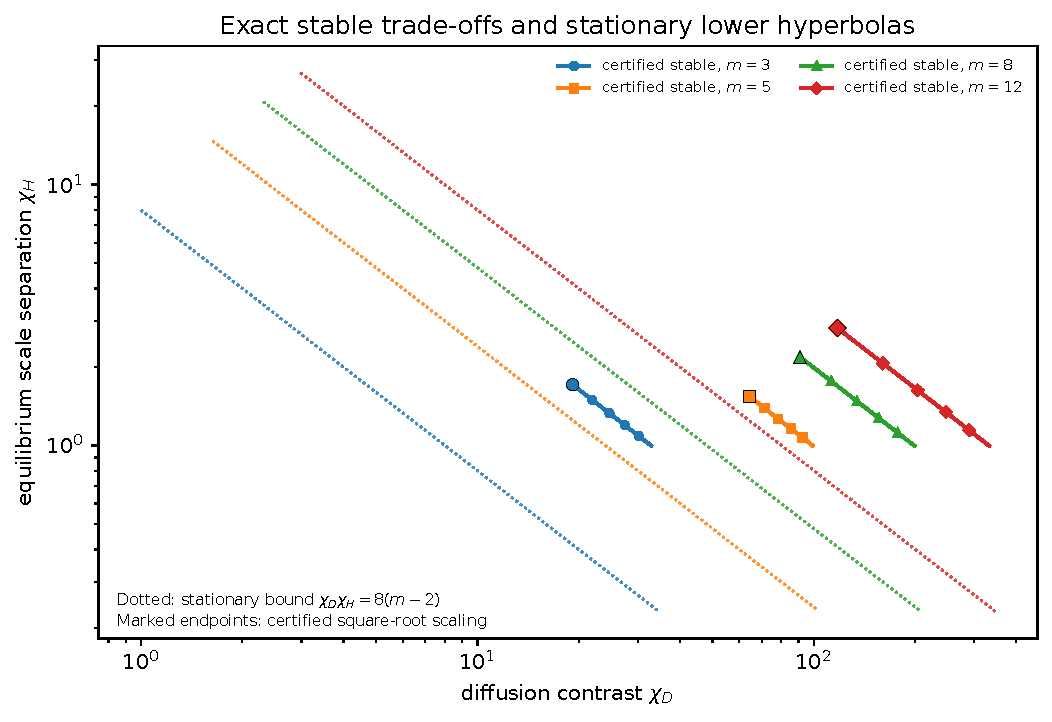
\includegraphics[width=.78\linewidth]{../figures/stable_tradeoff.pdf}
\caption{Exact heterogeneity trade-offs for representative dimensions.  The
dotted hyperbolas are the topology-specific necessary bounds for stationary
crossings of $\widehat N_m$, $\chi_D\chi_H=8(m-2)$; the solid curves are
certified stable families with product $23(91(m-2)-1)/63$.  Each marked point is the certified
square-root-scaling endpoint for its dimension.  Constants are not claimed
optimal.}
\label{fig:tradeoff}
\end{figure}

\section{The nonlinear frontier and finite-dimensional transparency}

The exact unit-equilibrium stable infimum is open.  The completed bounds are
\begin{equation}\label{eq:frontierbounds}
 8(m-2)\le\chi_{\rm stable}(m)
 \le\frac{23(91m-183)}{63}.
\end{equation}
A canonical near-threshold affine path, defined in Supplement Section~S9,
has, at $m=3$,
\begin{equation}\label{eq:nearcritical}
 c_3(\varepsilon)=\frac6{1379}+
 \frac{421985}{11409846}\varepsilon+O(\varepsilon^2),
 \qquad c_3(\varepsilon)>0\quad(0<\varepsilon\le10^{-3}).
\end{equation}
Thus approaching the sharp linear threshold does not automatically preserve
supercriticality.  This is a boundary example, not a universal nonlinear gap.

\begin{table}[t]
\centering
\small
\begin{tabular}{rrrrrrrrrr}
\toprule
$m$&$n$&$\chi_D^{\rm unit}$&$\chi_D^{\rm scale}$&$\chi_H^{\rm scale}$&product&lower&$\eta_m$&$c_m$&$\sqrt{-\eta_m/c_m}$\\
\midrule
3&4&32.8571&19.1809&1.71302&32.8571&2.82843&0.0192752&-0.00244362&2.80855\\
4&5&66.0794&27.1258&2.43603&66.0794&4&0.00992406&-0.00135495&2.70635\\
5&6&99.3016&33.2222&2.98901&99.3016&4.89898&0.00668208&-0.000932507&2.67689\\
6&7&132.524&38.3617&3.45458&132.524&5.65685&0.00503668&-0.000710298&2.66288\\
7&8&165.746&42.8897&3.86447&165.746&6.32456&0.00404149&-0.000573473&2.65469\\
8&9&198.968&46.9833&4.23487&198.968&6.9282&0.00337468&-0.000480799&2.64932\\
9&10&232.19&50.7478&4.57538&232.19&7.48331&0.00289675&-0.000413892&2.64553\\
10&11&265.413&54.2517&4.89225&265.413&8&0.0025374&-0.000363322&2.6427\\
\bottomrule
\end{tabular}

\caption{Current-profile diagnostics generated from one exact source.
$\chi_D^{\rm unit}$ is the current unit-equilibrium stable-profile contrast;
$\chi_D^{\rm scale}$ and $\chi_H^{\rm scale}$ are the physical contrasts at
the certified square-root-scaling endpoint; ``product'' is their exact product
$23(91(m-2)-1)/63$; ``lower'' is $\sqrt{8(m-2)}$; and $\eta_m$, $c_m$, and
$\sqrt{-\eta_m/c_m}$ use the current unit-profile normal-form convention.
The identity $\chi_D^{\rm unit}=\chi_D^{\rm scale}\chi_H^{\rm scale}$ is
exact, not a numerical coincidence.  The table is illustrative and proves no
all-dimensional claim.}
\label{tab:finite}
\end{table}

\begin{proposition}[Retuned local robustness]\label{prop:robust}
Fix $m$ and a certified $L$.  Sufficiently small perturbations within the
positive-equilibrium realization manifold---equivalently, of positive steady
fluxes and equilibrium coordinates with rates reconstructed accordingly---as
well as small perturbations of diffusion ratios and interval length, admit a
unique nearby scalar diffusion multiplier at which the primary supercritical
bifurcation and local exponential stability persist.
\end{proposition}

\begin{proof}
Continue the simple critical eigenvalue as a smooth function of the physical
parameters and one scalar diffusion multiplier.  Its multiplier derivative is
the nonzero transversality pairing.  The implicit function theorem gives the
nearby critical multiplier and equilibrium.  Homogeneous and finitely many
low-mode gaps persist by analytic perturbation.  In a common neighborhood,
a positive diffusion lower bound and a reaction-Jacobian upper bound control
all high modes.  The reduced normal-form coefficients and branch spectral
projection depend smoothly on parameters, so the negative cubic sign and
complementary branch gap persist.  One scalar multiplier is retuned; arbitrary
nearby parameter points are not asserted to be critical.
\end{proof}

\paragraph{Open problems.}
\begin{enumerate}[leftmargin=2em]
\item Determine whether $\chi_{\rm stable}(m)=8(m-2)$ as an infimum at unit
equilibrium.
\item Determine whether supercritical stable pattern formation has a strict
nonlinear contrast gap above the linear threshold.
\item Determine the constant-optimal stable diffusion--equilibrium frontier,
or equivalently the exact infimum of $\max(\chi_D,\chi_H)$.
\item Determine the exact threshold for oscillatory diffusion-driven
instability in this topology and whether wave instability can occur at lower
diffusion or heterogeneity contrast than the sharp stationary threshold.
\end{enumerate}

\section{Numerical illustrations}

The symbolic theorem does not use simulation.  We integrated cosine--Galerkin
systems for $m=3,5,8$ near the exact unit-equilibrium branches, extracted the
first-mode amplitude with the adjoint projection, and repeated the
calculations under spatial and temporal refinement.  Parameters, tolerances,
profiles, and open-format data accompany the code.

\begin{figure}[H]
\centering
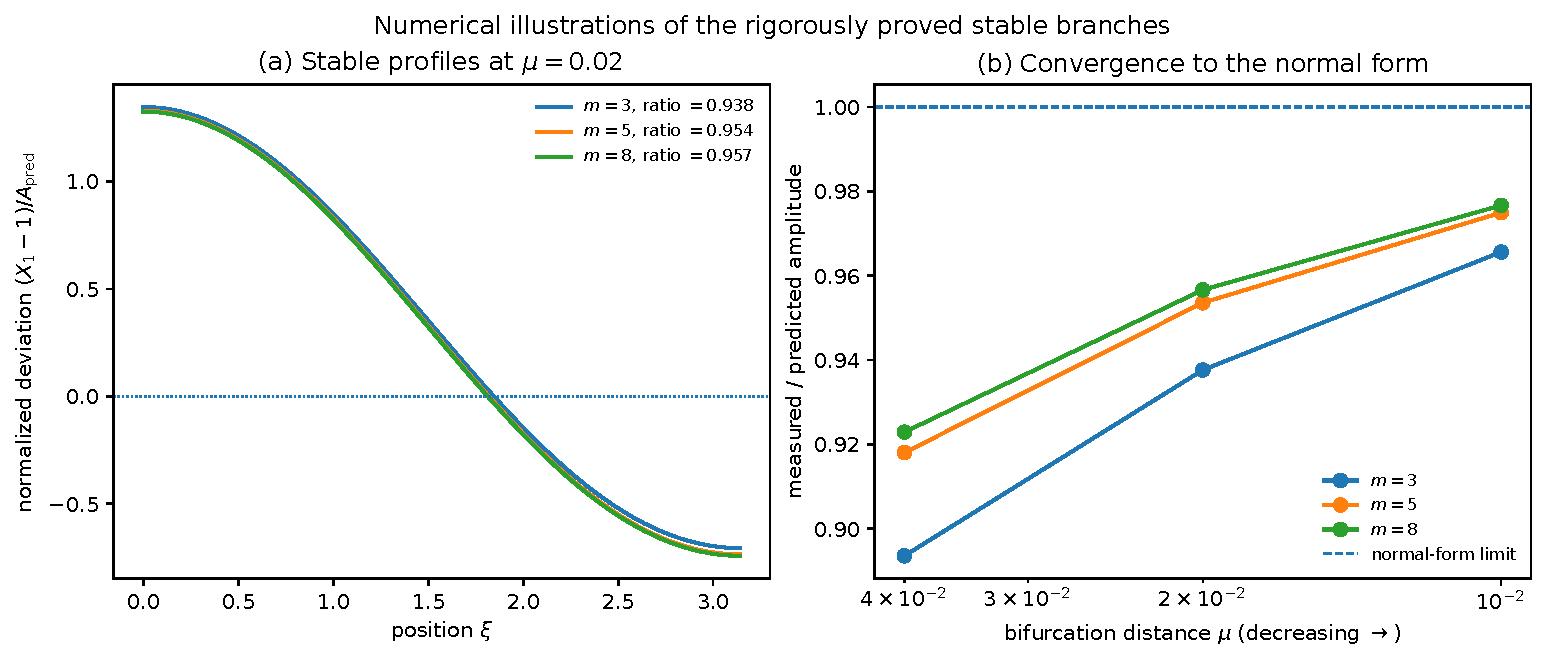
\includegraphics[width=.92\linewidth]{../figures/stable_profiles.pdf}
\caption{Numerical illustrations of the rigorously proved local patterned
branches.  Panel (b) compares the measured adjoint-projected amplitude
with $\sqrt{-\eta_m\mu/c_m}$.  Numerical illustrations are not used in any
proof.}
\label{fig:profiles}
\end{figure}

\section{Relation to prior work and limitations}

The possibility of order-$(n-1)$ unstable (activator) subsystems for general
fixed matrices is established in multicomponent Turing theory
\cite{Satnoianu2000}; that fixed-matrix possibility is not claimed as new.
Anma, Sakamoto, and Yoneda give complementary three-component
unstable-subsystem analysis \cite{Anma2012}.  The present distinction is the
conjunction of one indexed
binary-complex classical mass-action topology, every positive rate and
equilibrium realization, all-spectrum stability of every smaller principal
block, exact diffusion design, and stable nonlinear patterned branches in
every dimension.

Haas and Goldstein quantified diffusion thresholds statistically for random
Jacobians through six components and found that many sampled instabilities
cannot be reduced to fewer diffusing species \cite{HaasGoldstein2021}.  Here
the scope is deterministic and complementary: one constrained mass-action
topology is treated exactly in every dimension, with all positive
realizations quantified and nonlinear branch stability proved.

Mincheva and Craciun's principal projected-network injectivity condition is a
different reaction-network notion and is not identified with principal-block
Hurwitz localization \cite{MinchevaCraciun2013}.  Interaction-topology and
atlas studies identify broad structural features and finite collections of
Turing-capable networks \cite{Marcon2016,Diego2018,Scholes2019}; the present
result instead gives one exact infinite topology family and a theorem uniform
over all positive realizations.
Marcon and collaborators showed that some architectures can pattern with
equally diffusing signals under their modeling assumptions \cite{Marcon2016}.
For the present topology, equal diagonal diffusion cannot destabilize: it only
shifts the homogeneous spectrum left.  Instead, the required stationary
heterogeneity is quantified exactly by \eqref{eq:criterion}; at unit
equilibrium its contrast floor is $8(m-2)$, and with equilibrium scaling the
topology-specific stationary heterogeneity requirement is
\eqref{eq:productlower}.  This is a complementary,
topology-specific quantitative result about differential-diffusion tuning, not
a statement about all binary-complex networks.  Parameter-rich unstable cores
allow derivative
freedoms absent from classical mass action \cite{VassenaStadler2024}.
Exact necessary-and-sufficient linear criteria for Turing and Turing--Hopf
instabilities in general three-species systems address a different
fixed-dimension scope \cite{Piskovsky2025}.  Complementarily,
Villar-Sep\'ulveda, Champneys, and Krause design Turing and wave instabilities
of prescribed wavelength by choosing a generally non-diagonal diffusion
tensor at fixed linearized kinetics, or conversely choosing linearized
kinetics at fixed transport \cite{VillarChampneysKrause2025}; here diffusion
is positive diagonal self-diffusion, and the Jacobians arise from---and are
quantified over---all positive-equilibrium realizations of one indexed
classical mass-action topology.  Biochemical screens study interpretable reaction
architectures rather than the synthetic extremal design here
\cite{Paul2024}.  Monomial-steady-state results give sufficient spatial
instability conditions for a restricted mass-action class
\cite{ConradiMinchevaUecker2026}.

The construction has one semipositive conservation law and an inflow; $X_1$
is not bounded by the conserved functional.  The local stability theorem does
not require an arbitrary-data global boundedness theorem.  All diffusivities
are positive and diagonal.  We do not treat immobile species, cross-diffusion,
projected-injectivity sharpness, weak reversibility, biochemical realization,
far-from-onset dynamics, global attraction, or dimension-uniform robustness.
The exact stable contrast constants remain open.

\section{Discussion}

The family is designed around two coupled positive-flux circuits.  Their
explicit two-parameter positive-flux factor $A_m(a,b)$, together with
arbitrary positive right-diagonal equilibrium scaling $H$, makes the
topology-wide quantifier tractable.  The long chain forces every unstable
principal subsystem to contain almost all species, while the boundary triad remains Hurwitz under
arbitrary positive equilibrium scaling.  The unique negative order-$(n-1)$
omission minor is the one omitting $Z$, which collapses stationary diffusion
design to one coefficient.  Finally, equilibrium scaling redistributes the
necessary heterogeneity between concentrations and physical diffusion without
changing the effective critical bracket or losing the negative cubic sign.
Along the certified scaled family, this is a contrast allocation rather than
a product reduction: $\chi_D(L)\chi_H(L)=\chi_D^{\rm unit}(m)$ is fixed while
$L$ reduces the larger of the two contrasts.

The resulting conclusion is both structural and quantitative.  The largest
proper unstable-subsystem order is unavoidable within this mass-action class;
the exact diffusion contrast is computable; stable positive patterns occur;
and diffusion and equilibrium contrasts can be controlled simultaneously at
the stationary-optimal square-root exponent for this topology.  The remaining
constant gap is explicit rather than
hidden and provides a focused nonlinear design problem.

\paragraph{Data and code availability.}
Exact certificates, independent verifiers, mutation tests, numerical data,
figure scripts, and replay instructions are frozen in the
\href{https://github.com/AlecKriebel/Math/tree/maximally-collective-stable-turing-v1.0.6/maximally_collective_stable_turing_patterns_binary_complex_mass_action_networks}{version 1.0.6 tagged release source tree}.
The versioned archive is indexed by the stable
\href{https://doi.org/10.5281/zenodo.21753404}{Zenodo concept DOI}.
The \href{https://github.com/AlecKriebel/Math/tree/main/maximally_collective_stable_turing_patterns_binary_complex_mass_action_networks}{mutable development source} remains on the main branch.

\paragraph{AI-assisted research disclosure.}
AI systems assisted with exploratory theorem discovery, symbolic derivation,
code generation, adversarial testing, proof organization, and prose editing.
AI systems are not authors.  The human author assumes responsibility for the
manuscript.  Central claims are supported by explicit proofs and independent
exact implementations; neither numerical agreement nor AI confidence is
treated as proof.

\begingroup
\renewcommand*{\bibfont}{\footnotesize}
\sloppy
\printbibliography
\endgroup
\end{document}
